\section{Solar irradiation\label{sec:externaldata_solar}}

The total solar irradiance $\Psi$ of the earth is defined as the incoming
solar energy at the top of the atmosphere per area, normed to a
sun--earth distance of 1~astronomical unit, and integrated over the
whole range of wavelengths $\left[0,\infty\left[\right.\right.$
(units: W/m$^2$).
The solar irradiance $\lambda\mapsto\psi(\lambda)$ is the incoming
solar energy at the top of the 
atmosphere per area and wavelength of electromagnetic radiation, also
normed to a sun--earth distance of 1~astronomical unit (units: W/m$^2$/nm). 
Solar irradiance $\psi$ and therefore $\Psi$ vary with time. The
variation patterns depend on 
the wave length and are therefore different for the various spectral
bands of \echam. For the old 6--band radiation scheme of ECHAM5, only the total
solar irradiance $\Psi$ was prescribed and the distribution onto the spectral
bands was fixed. This means that for a spectral band
$[\lambda_1,\lambda_2]$, the incoming energy
\begin{displaymath}
\psi_{\lambda_1,\lambda_2}:=\int\limits_{\lambda_1}^{\lambda_2}\psi(\lambda)\,d\lambda 
\end{displaymath} 
was determined from fixed fractions
$\xi_{\lambda_1,\lambda_2}:=\psi_{\lambda_1,\lambda_2}/\Psi$. For the
new 14--band SRTM 
radiation scheme implemented in \echam{} (section~\ref{sec_shortwave}),
the incoming solar irradiance of each band 
$\psi_{\lambda_1,\lambda_2}$ can vary independently with time.



\subsection{Historic}

\begin{sloppy}
For historic and future solar irradiance data we follow as closely as
possible the recommendations 
for CMIP5 as provided by the SPARC/SOLARIS project as  given on the
web site ({\tt
  http://www.geo.fu-berlin.de/en/met/ag/strat/forschung/SOLARIS/Input\_data/}
\\ 
{\tt CMIP5\_solar\_irradiance.html}).
Historic data for the period 1850 until 2008 was reconstructed based
on observations and proxy data by J. Lean (Naval Research Laboratory,
Washington D.C., USA). Detailed information on the reconstruction is
provided at the above mentioned web site.  
Total solar irradiance variations were reconstructed as described by
\citet{froehlich_04} based on time series of sunspots and faculae. 
The spectral dependence of the solar irradiance and its variability
was determined from the 
spectral dependence of the sunspot blocking and 
facular brightening, as described in detail by \citet{lean_00}. 
Data are provided for wavelengths from 100 to 100000 nm with a
spectral resolution of 1 nm for small  
wavelengths and increasing with wavelength. For use in \echam{} the
original data have been averaged over the wavelength bins of  
the SRTM code as given in table~\ref{tab_srtm} and scaled in order to
provide the full TSI in the wavlength range covered by the SRTM
scheme. 
Additionally, as recommended by SPARC/SOLARIS, the orginal data have
been multiplied by 
a factor of 0.9965. This was done in order to obtain a TSI close 
to 1361 W/m$^2$ as suggested by recent observations instead of about
1368 W/m$^2$ assumed earlier. 
The temporal resolution of the original data is annually until 1881
and monthly starting in 1882. 
For use in \echam{} we have linearly interpolated the annual data
available before 1882 to monthly values in order to 
provide consistent data sets over the full historic period. However,
it should be kept in mind that short period variability of solar
irradiance 
used as input in the CMIP5 simulations is larger after than before
1882 (see Fig.~\ref{fig:eps}). 
\end{sloppy}

\subsection{Scenarios}
For the future scenarios it is recommended to repeat solar cycle 23, i.e. irradiance data of the period 
May 1996 to July 2008 for August 2008 to Oct 2020, Nov 2020 to Jan 2033, etc. 
This means that data files for the 49 years from 2008 to 2056 can be used as input for the years 2057 to 2105 and 
further repeated for later periods. The time series of monthly TSI integrated from the spectral irradiances used for
the period 1850--2100 is presented in Fig.~\ref{fig:eps}.


Monthly averaged spectral irradiance data for the years 1850--2100 are stored in yearly files
{\tt swflux\_14band\_yyyy.nc}, {\tt yyyy} being the year.
These files contain the monthly mean values of $\Psi$ as {\tt TSI} and
$\psi_{\lambda_1,\lambda_2}$ as {\tt SSI} in W/m$^2$. These variables
are read into \echam{} and linearly interpolated with respect to time to
the actual model radiation time step.






\begin{figure}[htb]
\[
\ifpdf
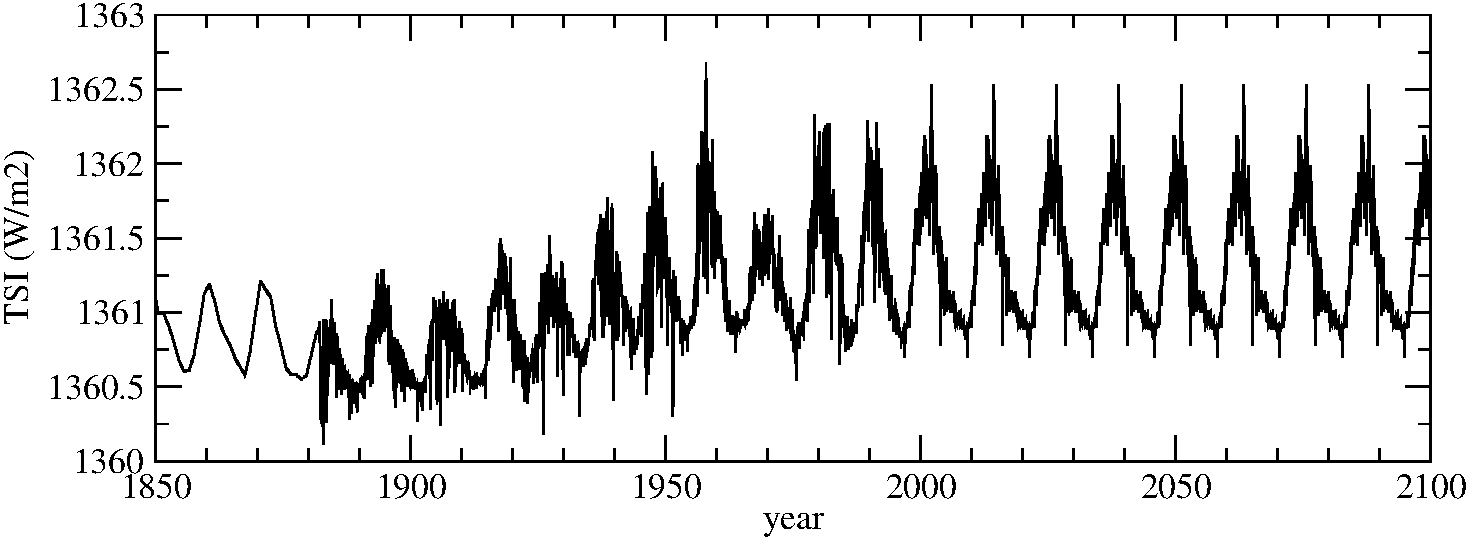
\includegraphics[width=15cm]{externaldata/tsi_1850-2100.pdf}
\else
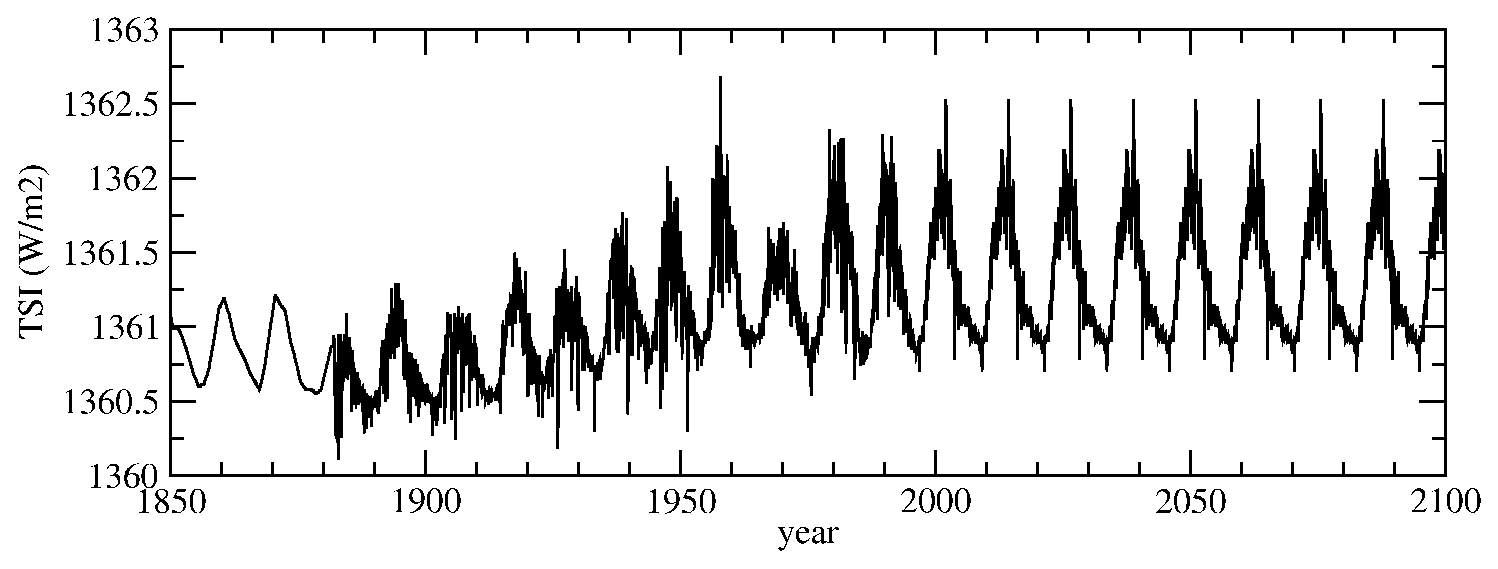
\includegraphics[width=15cm]{externaldata/tsi_1850-2100.eps}
\fi
\]
\caption{\label{fig:eps}Monthly averaged total solar irradiance (TSI) resulting from the spectrally resolved irradiance used in CMIP5
simulations with \echam.}
\end{figure}

\subsection{Climatologies}

Several choices of climatological solar irradiance (i.e.~constant solar
irradiance that is independent of time) are available: The
original ``SRTM'' values, a solar irradiance averaged over the years
1844--1856 (``preindustrial'') 
that was used in the preindutrial control simulations of CMIP5, 
and a solar irradiance averaged over the years 1979--1988 (``amip'').
In the latter two cases averaging was performed over data from the
time dependent historic data set as described below. 
For simulations with constant solar irradiance it is recommended to
use the ``preindustrial'' or ``amip'' 
climatological values which provide total solar irradiances (TSI) of
close to 1361 W/m$^{2}$ to which \echam{} has been tuned. 
The original TSI of ``SRTM'' is of about 1368 W/m$^{2}$ (see
table~\ref{tab_srtm}). 
All the mentioned climatologies do not have to be read in from
external files but can be accessed by specific choices 
of namelist parameters.


\begin{table}[hb]
\caption{$\psi_{\lambda_1,\lambda_2}$ in $\rm W/m^2$ as defined for the original
SRTM radiation scheme (SRTM), for the preindustrial period (preind),
and the amip period (amip). The resulting total solar irradiance
(solar 
constant) $\Psi$ is $1368.222\,{\rm W/m^2}$ for the original SRTM
scheme, $1360.875\,{\rm W/s^2}$ for the preindustrial period, and
$1361.371\,{\rm W/m^2}$ for the amip period.}\label{tab_srtm} 
\begin{tabular*}{\textwidth}{c@{\extracolsep\fill}cccc}\hline\hline
band/nm & 3077 --\cw{0}3846&2500 --\cw{0}3077&2151 --\cw{0}2500&1942 --\cw{0}2151\\
index & 1 & 2 & 3 & 4 \\
$\psi_{\lambda_1,\lambda_2}$ (SRTM) 
& \cw{0}12.1096\cw{0} & \cw{0}20.3651\cw{0} & \cw{0}23.7297\cw{0} &\cw{0}22.4277\cw{0}\\
$\psi_{\lambda_1,\lambda_2}$ (preind) 
& \cw{0}11.9500\cw{0} & \cw{0}20.1461\cw{0} & \cw{0}23.4030\cw{0} &\cw{0}22.0944\cw{0}\\
$\psi_{\lambda_1,\lambda_2}$ (amip) 
& \cw{0}11.9505\cw{0} & \cw{0}20.1477\cw{0} & \cw{0}23.4039\cw{0} &\cw{0}22.0946\cw{0}\\\hline
band/nm & 1626 --\cw{0}1942&1299 --\cw{0}1626&1242 --\cw{0}1299&\cw{0}788 --\cw{0}1242\\
index & 5 & 6 & 7 & 8 \\
$\psi_{\lambda_1,\lambda_2}$ (SRTM) 
& \cw{0}55.6266\cw{0} & 102.932\cw{00} & \cw{0}24.2936\cw{0} &345.742\cw{00}\\
$\psi_{\lambda_1,\lambda_2}$ (preind) 
& \cw{0}55.4168\cw{0} & 102.512\cw{00} & \cw{0}24.6954\cw{0} &347.472\cw{00}\\
$\psi_{\lambda_1,\lambda_2}$ (amip) 
& \cw{0}55.4140\cw{0} & 102.513\cw{00} & \cw{0}24.6981\cw{0} &347.536\cw{00}\\\hline
band/nm&\cw{0}625 --\cw{00}788&\cw{0}442 --\cw{00}625&\cw{0}345 --\cw{00}442&\cw{0}263 --\cw{00}345\\
index & 9 & 10 & 11 & 12 \\
$\psi_{\lambda_1,\lambda_2}$ (SRTM) 
& 218.187\cw{00} & 347.192\cw{00} & 129.495\cw{00} &\cw{0}50.1522\cw{0}\\
$\psi_{\lambda_1,\lambda_2}$ (preind) 
& 217.222\cw{00} & 343.282\cw{00} & 129.300\cw{00} &\cw{0}47.0762\cw{0}\\
$\psi_{\lambda_1,\lambda_2}$ (amip) 
& 217.292\cw{00} & 343.422\cw{00} & 129.403\cw{00} &\cw{0}47.1426\cw{0}\\\hline
band/nm & \cw{0}200 --\cw{00}263&3846 --12195&&\\
index & 13 & 14 &  &  \\
$\psi_{\lambda_1,\lambda_2}$ (SRTM) 
& \cw{00}3.07994 & \cw{0}12.8894\cw{0} & &\\
$\psi_{\lambda_1,\lambda_2}$ (preind) 
& \cw{00}3.17212 & \cw{0}13.1807\cw{0} & &\\
$\psi_{\lambda_1,\lambda_2}$ (amip) 
& \cw{00}3.17213 & \cw{0}13.1808\cw{0} & &\\\hline\hline
\end{tabular*}
\end{table}
